% Copyright (C) 2012 Thomas L. Kula
% All Rights Reserved
%
% See the file LICENSE for license terms.
\documentclass[12pt]{article}
\usepackage{graphicx}
\usepackage{rotating}
\usepackage{fix-cm}
\usepackage{multirow}
\setlength{\paperwidth}{5.5in}
\setlength{\paperheight}{8.5in}
\setlength{\textheight}{7.45in}
\setlength{\topmargin}{-1.0in}
\setlength{\oddsidemargin}{-0.5in}
\setlength{\evensidemargin}{-0.5in}
\setlength{\textwidth}{4.0in}
\setlength{\parindent}{0in}
\setlength{\parskip}{3mm}
\usepackage[print]{booklet} \nofiles
\source{\magstep0}{5.5in}{8.5in}
\target{\magstep0}{11in}{8.5in}
\setpdftargetpages
\pagestyle{empty}
\begin{document}


\begin{center}
{\fontsize{36}{48}\selectfont \textsc{Haiku a Day }}
\end{center}

\vspace*{3.5cm}

{\fontsize{20}{40}\selectfont 

The drone of fans turn ---

As the weather grows colder ---

Radiator glug


}

\vspace*{5.0cm}
\begin{center}
{\large{Issue 87: September 2012}} \\[5mm]
{\fontsize{8}{8}\selectfont  \textsc{ St. Joshua Norton Press }} \\[1mm]
{\fontsize{6}{6}\selectfont Mathom House by the Cloisters \textbar The People's Republic of Ames }
\end{center}


\newpage

I have had cider and doughnuts. This makes me a very
happy man.

--- Thomas

http://kula.tproa.net/had/ \\
kula@tproa.net

Download this and previous HADs at the website, so you can
print out your own (DIY, yeah!) or if you want me to send
you one, send me your address, and maybe a stamp if you
are feeling nice. Or send me something you've made ---
trades always appreciated, postcards are nice too.

\vfill

1 September 2012

Need a stasis field \\
For the food stuck in my fridge; \\
It goes bad too soon

2 September 2012

Some music, blasting \\
Comes through my open window \\
I hate all of you

\newpage

3 September 2012

A quiet morning \\
Black coffee, quiet reading \\
Some haiku, and you

4 September 2012

A mental model \\
Of how some shelves should be built. \\
Now reality?

5 September 2012

With a tick, a leaf \\
Starts its breakdown, on the ground \\
Returning to it

6 September 2012

Even when cooking \\
The word `rub', vaguely dirty \\
Bothering my mind

7 September 2012

Not all things are neat \\
Some stories lack a moral \\
Some just lack a plot

8 September 2012

Nearly a year gone \\
And this door still annoys me. \\
Memo: sandpaper

9 September 2012

Rounding a corner \\
I see a dog with balloons \\
I need more coffee

\newpage

10 September 2012

The rumble tumble \\
Is no place for weakened ones: \\
Nifty socks die first

11 September 2012

From an old party \\
A laurel wreath, on a shelf, \\
Shedding dry bay leaves

12 September 2012

With repetition \\
You slowly drag a new skill \\
To experienced

13 September 2012

Dinner in the park \\
A pleasant evening walk \\
This day ended well

14 September 2012

In case of fire \\
I swear I didn't do it \\
You'll never catch me!

15 September 2012

Vortex of noisy \\
Being shuffled back and forth \\
Makes the carpet clean

16 September 2012

On a wave of light \\
Color, streaming from the Sun \\
Warming the sidewalk


\newpage

17 September 2012

You may talk the talk. \\
You may even walk the walk. \\
Do you sit the sit?

18 September 2012

Struggle with the seal \\
The pickle jar, suddenly \\
Opens, briney splash

19 September 2012

A boom from outside \\
Someone's car hit a light post \\
Flashy lights ensue

20 September 2012

An ancient well sits--- \\
That's not true, it doesn't sit. \\
An ancient well deeps.

21 September 2012

Anniversary. \\
There should be a party for \\
That word's creation

22 September 2012

High voltage. Ozone. \\
The hum of transformers, low. \\
Weird infrastructure.

23 September 2012

That box a mistake \\
Stuff I shouldn't have but keep \\
Throw away? No, store.


\newpage

24 September 2012

When I'm dictator, \\
There will be a penalty \\
For cell phones on stairs

25 September 2012

Why does grapefruit juice \\
Seem like it's tasty to me, \\
After years of hate?

26 September 2012

There's territory, \\
Not organization here. \\
Clouds of stuff, not shelves.

27 September 2012

A daily crossing \\
And an eternal question: \\
Will I beat the train?

28 September 2012

Going in reverse \\
I eat dessert first, because \\
Life is uncertain

29 September 2012

Unhappy damp towel \\
Works poorly to dry dishes \\
Get another one

30 September 2012

Ponder overhead \\
The trillions of molecules \\
Pounding on your skull

\newpage

\begin{center}
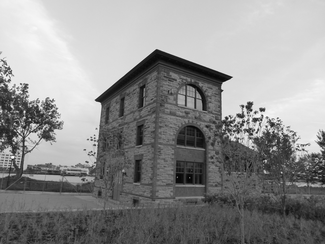
\includegraphics[width=325pt]{roosevelt.png}
Strecker Memorial Laboratory, Roosevelt Island \\
17 September 2012
{\tt kula.tproa.net/photos/2012/20120917-roosevelt-island/ }

\end{center}

\newpage

\thispagestyle{empty}
\vspace*{12cm}
\begin{sideways}
\Large{St. Joshua Norton Press}
\end{sideways}
\begin{sideways}
\Large{PO Box 250138}
\end{sideways}
\begin{sideways}
\Large{New York NY 10025}
\end{sideways}


\end{document}


